\documentclass{article}
\usepackage[spanish]{babel} %Definir idioma español
\usepackage[utf8]{inputenc} %Codificacion utf-8
\usepackage{amssymb, amsmath, amsbsy, wasysym}
\usepackage{multirow} % para tablas
\usepackage{graphicx}
\usepackage[dvipsnames]{xcolor}
\title{Práctica 6}
\author{Emmanuel Peto Gutiérrez}
\begin{document}
\maketitle

\section{Introducción}

Esta práctica consiste en implementar el algoritmo de \emph{Dijkstra} para obtener el árbol de rutas más cortas de una gráfica.

A continuación se presenta un pseudocódigo para el algoritmo.

\begin{itemize}
\item $w(u,v)$: representa el peso de la arista $(u,v)$.
\item $Q$: cola de prioridad.
\item $G.V$: conjunto de vértices de la gráfica $G$.
\item $s$: vértice de origen.
\item $G.Adj[u]$: vecindad de $u$.
\end{itemize}

Dijkstra($G$,$s$)\\
\phantom{1}1 {\bf for} each vertex $v \in G.V$\\
\phantom{1}2 \hspace{5mm}$v.d = \infty$\\
\phantom{1}3 \hspace{5mm}$v.p = null$\\
\phantom{1}4 $s.d = 0$\\
\phantom{1}5 $Q = G.V$\\
\phantom{1}6 {\bf while} $Q \not = \emptyset$\\
\phantom{1}7 \hspace{5mm}$u = Q.extract\_min()$\\
\phantom{1}8 \hspace{5mm}{\bf for} each vertex $v \in G.Adj[u]$\\
\phantom{1}9 \hspace{10mm}{\bf if} $v.d > u.d + w(u,v)$\\
10 \hspace{15mm}$v.d = u.d + w(u,v)$\\
11 \hspace{15mm}$v.p = u$

\section{Descripción}

\subsection{Entrada}

El programa debe recibir como entrada el nombre del archivo de texto que contiene la información necesaria para construir la gráfica $G$. Esto es:

$\bullet$ En la primera línea, los vértices(representados por números) separados por comas.

$\bullet$ De la segunda línea en adelante, tripletas de números separados por comas: $a,b,w$. El primer número representa el vértice $a$, el segundo el vértice $b$ y el tercero el peso de la arista $(a,b)$.

También debe recibir el vértice de origen como un número.

\subsection{Salida}

Se debe imprimir la distancia entre el vértice de origen y el resto de los vértices. Además, se debe imprimir el camino a recorrer del vértice $s$ a cada vértice $v$.

Por ejemplo, para la siguiente gráfica:

\includegraphics[scale=0.7]{dibujos/grafica}

el resultado de aplicar el algoritmo con raíz $v_0$ es el siguiente:

\includegraphics[scale=0.7]{dibujos/grafica2}

Así que el programa debe imprimir algo como esto:\\
$\bullet$ v1, 4 $\rightarrow$ [v0, v1]\\
$\bullet$ v2, 12 $\rightarrow$ [v0, v1, v2]\\
$\bullet$ v3, 19 $\rightarrow$ [v0, v1, v2, v3]\\
$\bullet$ v4, 21 $\rightarrow$ [v0, v7, v6, v5, v4]\\
$\bullet$ v5, 11 $\rightarrow$ [v0, v7, v6, v5]\\
$\bullet$ v6, 9 $\rightarrow$ [v0, v7, v6]\\
$\bullet$ v7, 8 $\rightarrow$ [v0, v7]\\
$\bullet$ v8, 14 $\rightarrow$ [v0, v1, v2, v8]

\section{Detalles}

La práctica debe ser implementada en Java. La cola de prioridad debe ser implementada con {\bf cola binomial}.

\section{Extra}

Se obtendrá un punto extra si se pintan de rojo las aristas que pertenecen al árbol de distancias.

\section{Entrega}

\begin{itemize}
\item Deben entregarlo como un archivo comprimido de una carpeta con el mismo nombre.
\item La carpeta debe ser: \textbf{Practica6\_ApellidopaternoApellidomaterno}. Por ejemplo \textbf{Practica6\_PetoGutierrez}.
\item Su carpeta debe contener un archivo \emph{readme} que contenga: número de cuenta, nombre completo, 
correo y las instrucciones para compilar y ejecutar su programa(se recomienda un \emph{Makefile}).
\item Si su carpeta contiene un ejecutable(como *.jar) enviarlo como un enlace de dropbox o drive.
\item El asunto debe ser: \textbf{[AAlgoritmos]Practica6}.
\item El correo al que enviarán la práctica es: \emph{empg014@ciencias.unam.mx}
\end{itemize}

La fecha de entrega es el \textbf{22 de noviembre}.

\end{document}